\section{Modele celowania w grach (Bartosz Strzelecki)}\label{s:cel}
Celowanie w grach taktycznych jest podstawowym elementem programu, który ma
olbrzymi wpływ na przebieg rozgrywki. Ten mechanizm jest przede wszystkim wykorzystywany
do wzbogacenia gry o kolejną warstwę decyzji taktycznych i zarządzania podejmowanym ryzykiem.
Gracz, przed oddaniem strzału, podejmuje decyzję czy warto zaryzykować podjęcie strzału o niskiej szansie
na trafienie, czy lepiej wykonać niezawodny atak, prawdopodobnie wystawiając się na ataki przeciwników.

W \textit{Phoenix Point}\footnote{\url{https://phoenixpoint.info}} modelowanie celności to wieloaspektowy system, który w zawiły sposób definiuje wynik interakcji bojowych.
Gra wykorzystuje dynamiczny system celowania, który uwzględnia różne elementy, takie jak postawa żołnierza, biegłość w posługiwaniu się bronią, zasięg, 
osłona i warunki środowiskowe, aby określić precyzję strzału. Każdy z tych elementów odgrywa znaczącą rolę w ogólnym obliczeniu trafienia w cel.

W przeciwieństwie do podobnej gry \textit{XCOM}\footnote{\url{https://www.xcom.com}}, gdzie celność jest zamodelowana za pomocą prostej szansy na trafienie, w grze \textit{Phoenix Point}
trajektoria każdego pocisku obliczana jest osobno. Podczas celowania widoczne są dwa okręgi: wewnętrzny, który reprezentuje miejsce,
w którym znajdzie się 50\% pocisków oraz zewnętrzny, który reprezentuje maksymalny rozrzut broni. W tym przypadku im celniejsza broń tym
okręgi będą mniejsze.

\begin{figure}[h]
\centering
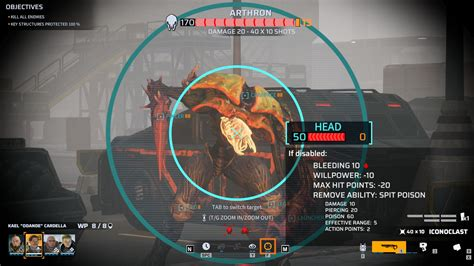
\includegraphics[width=1\textwidth]{images/point}
\caption[System celowania występujący w grze \textit{Phoenix Point}]{System celowania występujący w grze \textit{Phoenix Point}\protect\footnotemark.}
\label{fig:acc}
\end{figure}
\footnotetext{Internet, \url{https://www.pcgamesn.com/wp-content/uploads/2019/12/phoenix-point-aim.jpg}, dostęp: 16.08.2023}
\FloatBarrier
Ostatecznie system zaimplementowany w grze \textit{Phoenix Point} okazuje się dużo bardziej realistyczny i pozwala na utrzymywanie ciągłej niepewności
co do celności strzału, umożliwiając w ten sposób na strategiczne wyzwania, leżących u podstaw gier tego typu. 
